% \section{Experimental Setup \& Model Benchmarking}
% \label{sec:comparison}

% To rigorously evaluate the proposed YOLO11-MobileNetV4 architecture against existing baselines, we established a comprehensive experimental environment focusing on data diversity and hardware constraints typical of automotive embedded systems.

% \subsection{Datasets}
% We utilized our dataset to train and validate our models. This dataset was selected for its diverse capture conditions on traffic lights.
% \begin{itemize}
%     \item Class Distribution: The dataset comprises 1000 images annotated with three primary classes: Red, Yellow, and Green, and Traffic Lights.
%     \item Preprocessing: All input images were resized to $320 \times 320$ pixels to align with the YOLO architecture's input stride. Pixel values were normalized to the range $[0, 1]$.
%     \item Augmentation: To prevent overfitting and improve generalization, we applied the Mosaic augmentation technique during training. This method combines four training images into one, forcing the model to learn to detect objects at different scales and in partial occlusion contexts-a critical requirement for real-world traffic scenarios.
% \end{itemize}

% \subsection{Hardware Environment}

% The experiments were divided into two distinct phases: high-performance training and resource-constrained inference.

% \paragraph{Training Setup} Model training was conducted on a high-performance workstation to ensure rapid convergence.
% \begin{itemize}
%     \item Processor: Intel Core i5-14600KF (14 Cores 20 CPUs, up to 5.3 GHz)
%     \item GPU: NVIDIA GeForce RTX 4060 (8GB GDDR6)
%     \item RAM: 32GB DDR4
%     \item OS: Windows 11 Pro
%     \item Framework: PyTorch 2.x with CUDA support.
%     % \item{Configuration} Training was performed with a batch size of 128 for 100 epochs, utilizing Stochastic Gradient Descent (SGD) with an initial learning rate of 0.01.
% \end{itemize}


% \paragraph{Deployment (Edge) Setup}
% To simulate a resource-constrained edge environment, the trained models were deployed on an embedded computing unit. The target platform represents a typical low-cost edge device operating with CPU-only inference.
% \begin{itemize}
%     \item \textit{Target Device:} Raspberry Pi 5 without dedicated accelerators (TPU/GPU) or high-speed SSD storage
%     \item \textit{CPU:} Broadcom BCM2712, 2.4\,GHz quad-core 64-bit Arm Cortex-A76
%     \item \textit{Memory:} 8\,GB RAM
%     \item \textit{Runtime:} Google LiteRT, CPU-only execution
% \end{itemize}


% \subsection{Comparative Model}

% To identify an efficient architecture for traffic light detection in embedded environments, we evaluated two distinct model configurations: the original YOLO11n and the YOLO11n–MobileNetV4 (ConvSmall). These models represent different points on the speed–accuracy trade-off, contrasting the higher detection precision of the baseline architecture with the improved computational efficiency of the lightweight backbone.

% \subsubsection{Accuracy}

% \begin{figure}[ht]
%     \centering
%     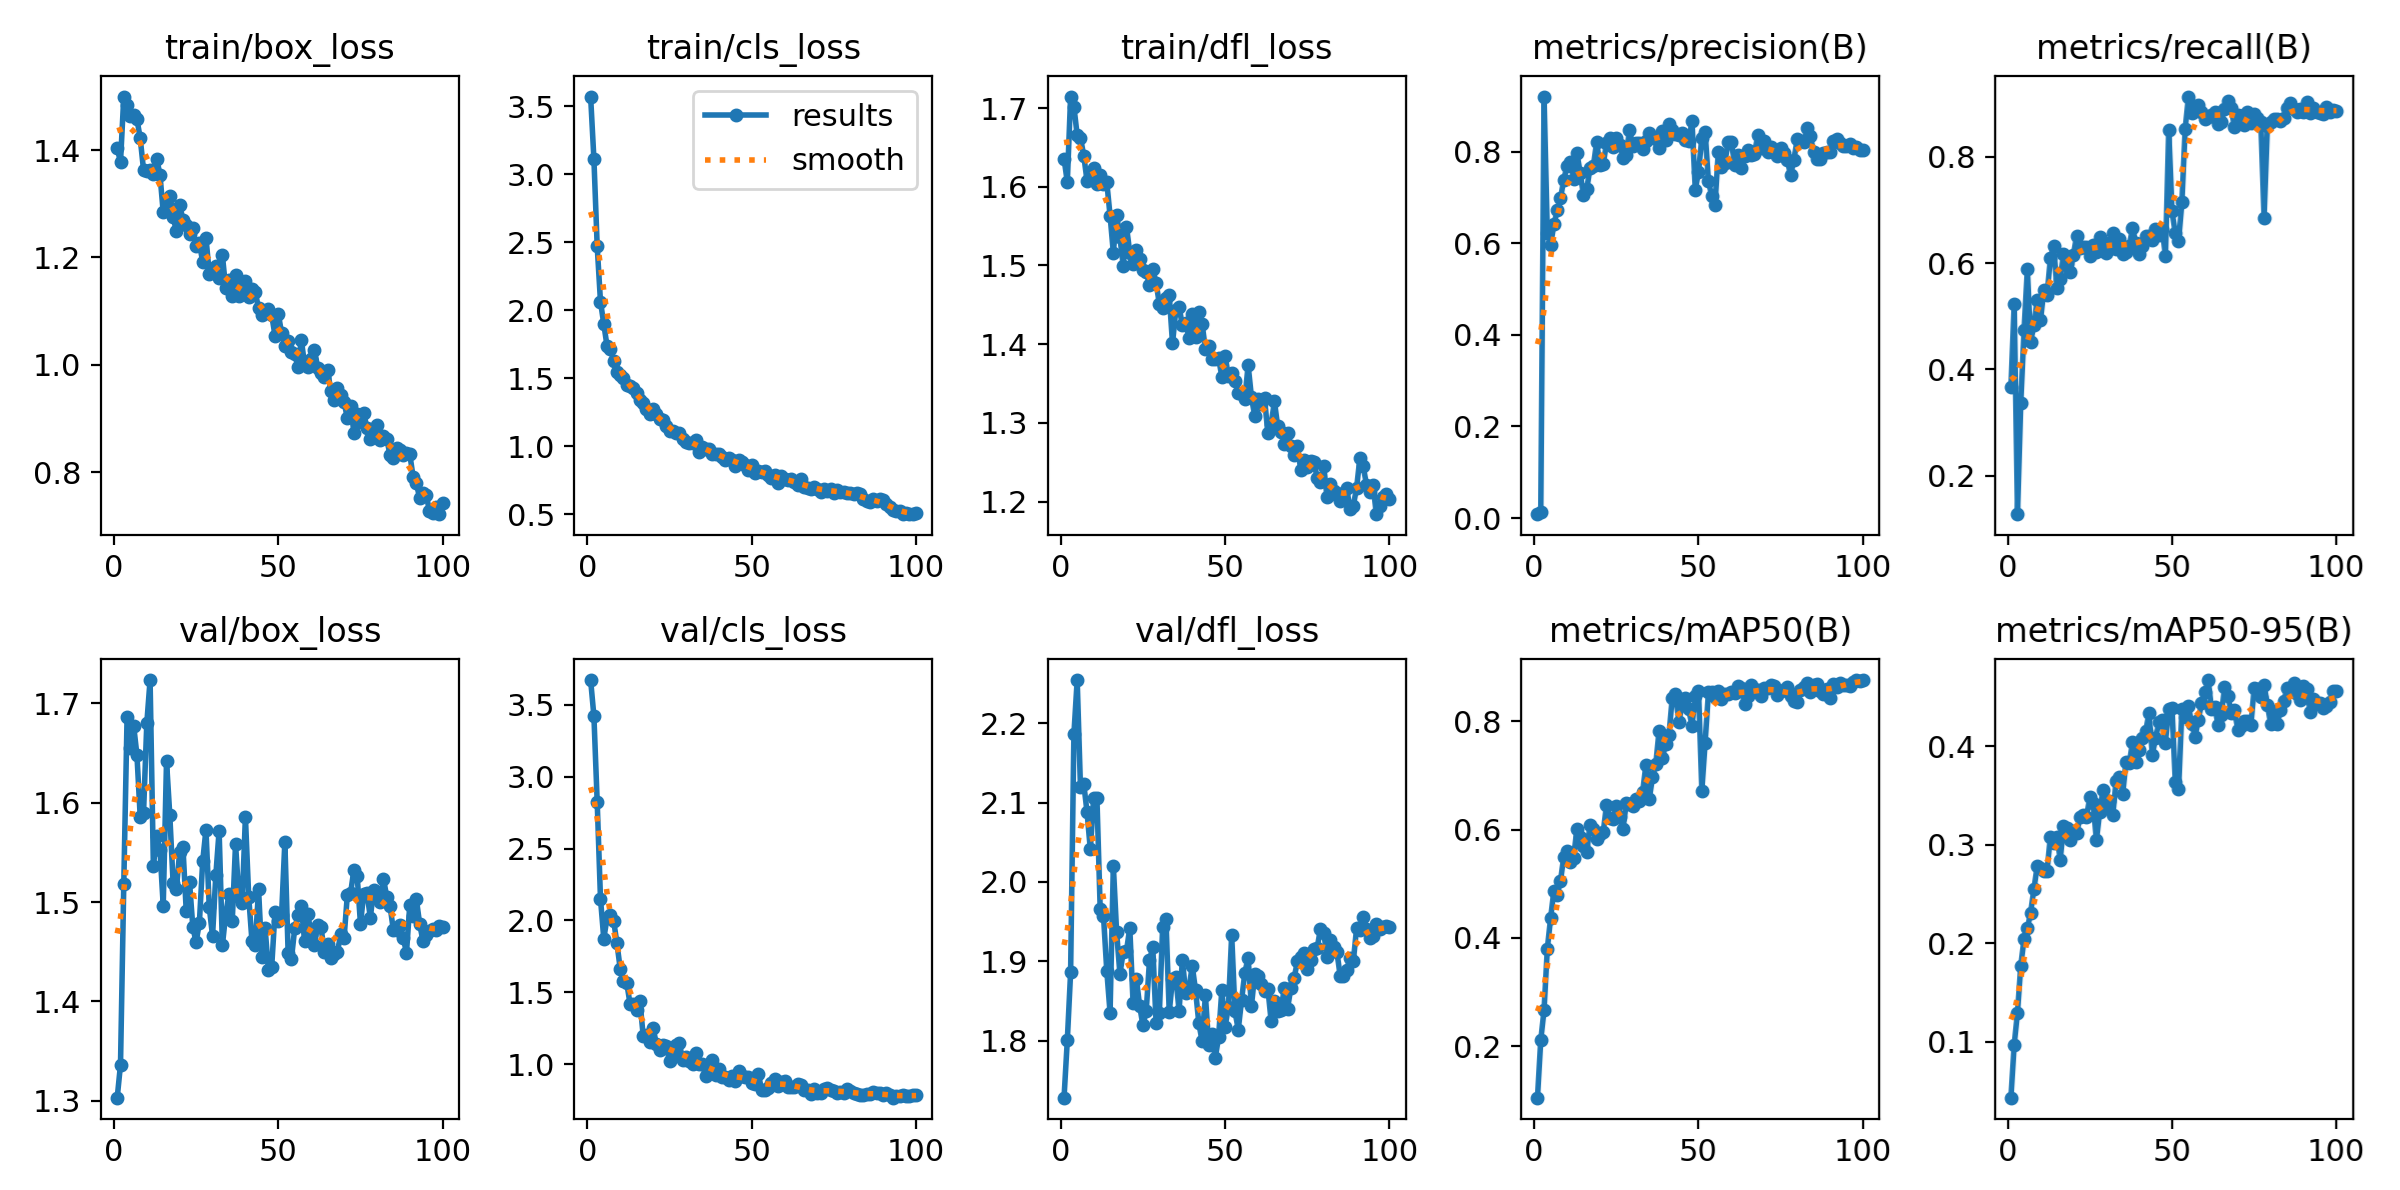
\includegraphics[width=1\linewidth]{Images/yolo11n_accuracy.png}
%     \caption{The accuracy of original YOLO11n}
%     \label{fig:yolo11n_accuracy}
% \end{figure}

% \begin{figure}[ht]
%     \centering
%     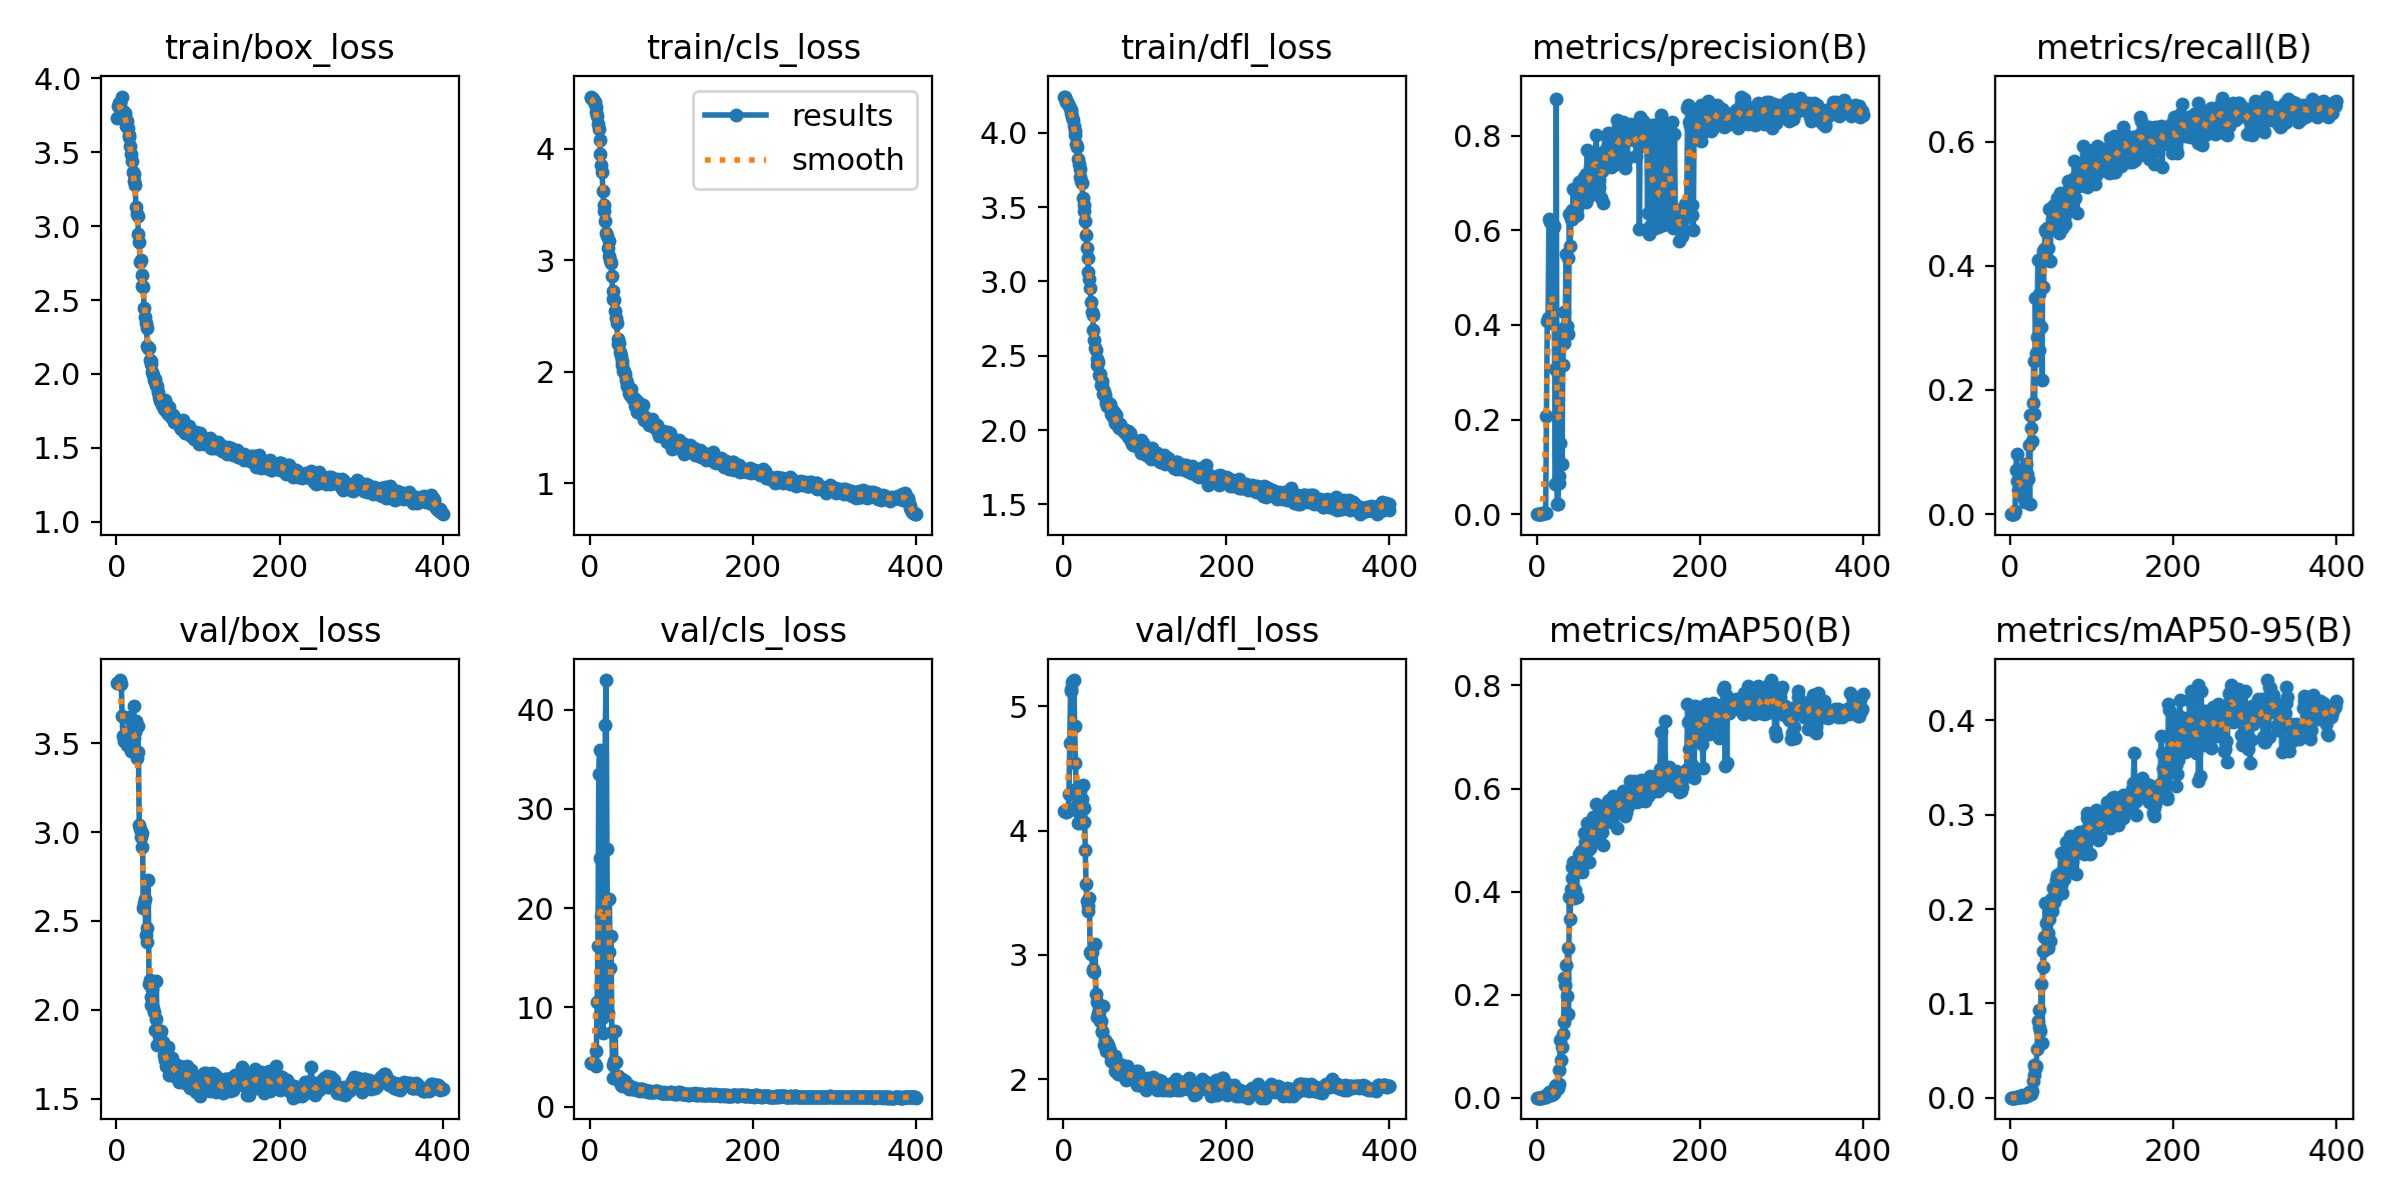
\includegraphics[width=1\linewidth]{Images/yolo11n-mbnv4accuracy.png}
%     \caption{The accuracy of YOLO11n-MobileNetV4ConvSmall}
%     \label{fig:yolo11n-mbnv4_accuracy}
% \end{figure}

% The training metrics presented in Fig. \ref{fig:yolo11n_accuracy} and Fig. \ref{fig:yolo11n-mbnv4_accuracy} illustrate the trade-off between the two architectures. The original YOLO11n backbone, with its robust feature extraction capabilities, achieves superior precision, outperforming the MobileNetV4 variant by approximately 10-15\% in both mAP@50 and mAP@50-95 metrics. 

% However, the MobileNetV4 variant demonstrates remarkable stability, retaining over 85\% of the baseline accuracy while significantly reducing model complexity. Although the lightweight backbone exhibits a slight degradation in precise object localization, the convergence curves indicate that the model remains highly effective for standard detection tasks. This result confirms that the MobileNetV4 architecture successfully exchanges a marginal fraction of accuracy for the computational efficiency required in resource-constrained environments.

% \subsubsection{Inference Speed}

% Inference latency is the critical bottleneck for deployment on the Raspberry Pi 5. Official benchmarks indicate that the original YOLO11n model (TFLite) requires over 400\,ms per inference on CPU, resulting in a non-real-time throughput of 2-3 FPS \cite{ultralytics_rpi5}.

% In contrast, our experimental results at Table \ref{tab:tradeoff_yolo_models} show that the YOLO11n-MobileNetV4 model reduces inference latency to 30-40ms. This represents a 90--92\% reduction in processing time, delivering a 10-13$\times$ speedup compared to the baseline. Consequently, the proposed architecture achieves a real-time frame rate of 25-33 FPS on generic embedded hardware, as illustrated in Fig.~\ref{fig:res_cpp}. This substantial efficiency gain-driven by the reduced parameter count of the MobileNetV4 backbone - validates its suitability for the Adaptive AUTOSAR edge node.

% \begin{table}[ht]
% \centering
% \caption{Trade-off comparison between YOLO11n and YOLO11n-MobileNetV4}
% \label{tab:tradeoff_yolo_models}
% \resizebox{\columnwidth}{!}{% % This scales the table to fit the column width
% \renewcommand{\arraystretch}{1.3}
% \begin{tabular}{|l|c|c|}
% \hline
% \textbf{Metric} & \textbf{YOLO11n (Original)} & \textbf{YOLO11n-MobileNetV4} \\ \hline
% Backbone & CSP-based YOLO & MobileNetV4 \\ \hline
% mAP@50 & Higher ($\approx$ 10--15\%) & Slightly lower \\ \hline
% mAP@50--95 & Higher ($\approx$ 10--15\%) & Slightly lower \\ \hline
% Precision / Recall & Marginally higher & Comp. / stable \\ \hline
% Inference (TFLite, CPU) & $>$400 ms & 30--40 ms \\ \hline
% Throughput (FPS) & 2--3 FPS & 25--33 FPS \\ \hline
% Speedup factor & 1$\times$ & $\approx$ 10--13$\times$ faster \\ \hline
% Inference reduction & -- & $\approx$ 90--92\% \\ \hline
% Complexity & Higher & Signif. reduced \\ \hline
% Edge Suitability & Limited & Highly suitable \\ \hline
% \textbf{Trade-off} & Higher accuracy & Speed balance \\ \hline
% \end{tabular}%
% }
% \end{table}




% % ----------------------------New section-------------------------
% \section{Experimental Setup and Model Benchmarking}
% \label{sec:comparison}

% This section evaluates the proposed YOLO11n-MobileNetV4 architecture against the original YOLO11n baseline, focusing on accuracy and inference performance under embedded hardware constraints.

% \subsection{Dataset}
% The models were trained and evaluated using a traffic light dataset containing diverse capture conditions.
% \begin{itemize}
%     \item \textit{Classes:} Red, Yellow and Green
%     \item \textit{Size:} approximately 6000 annotated images within argument
%     \item \textit{Preprocessing:} Images resized to $320 \times 320$ and normalized to $[0,1]$
%     \item \textit{Augmentation:} Mosaic augmentation applied during training to improve robustness to scale variation and partial occlusion
% \end{itemize}

% \subsection{Hardware Environment}
% Experiments were conducted in edge device.

% % \paragraph{Training Setup}
% % \begin{itemize}
% %     \item CPU: Intel Core i5-14600KF
% %     \item GPU: NVIDIA RTX 4060 (8GB)
% %     \item RAM: 32GB
% %     \item Framework: PyTorch with CUDA
% % \end{itemize}

% \paragraph{Deployment (Edge) Setup}
% \begin{itemize}
%     \item Device: Raspberry Pi 5 (CPU-only, no TPU/GPU)
%     \item CPU: Broadcom BCM2712, quad-core Arm Cortex-A76 @ 2.4\,GHz
%     \item Memory: 8GB RAM
%     \item Runtime: Google LiteRT
% \end{itemize}

% \subsection{Compared Models}
% Two configurations were evaluated to analyze the speed--accuracy trade-off for embedded traffic light detection:
% \begin{itemize}
%     \item YOLO11n (original backbone)
%     \item YOLO11n--MobileNetV4 (ConvSmall)
% \end{itemize}

% \subsubsection{Detection Accuracy}

% \begin{figure}[ht]
%     \centering
%     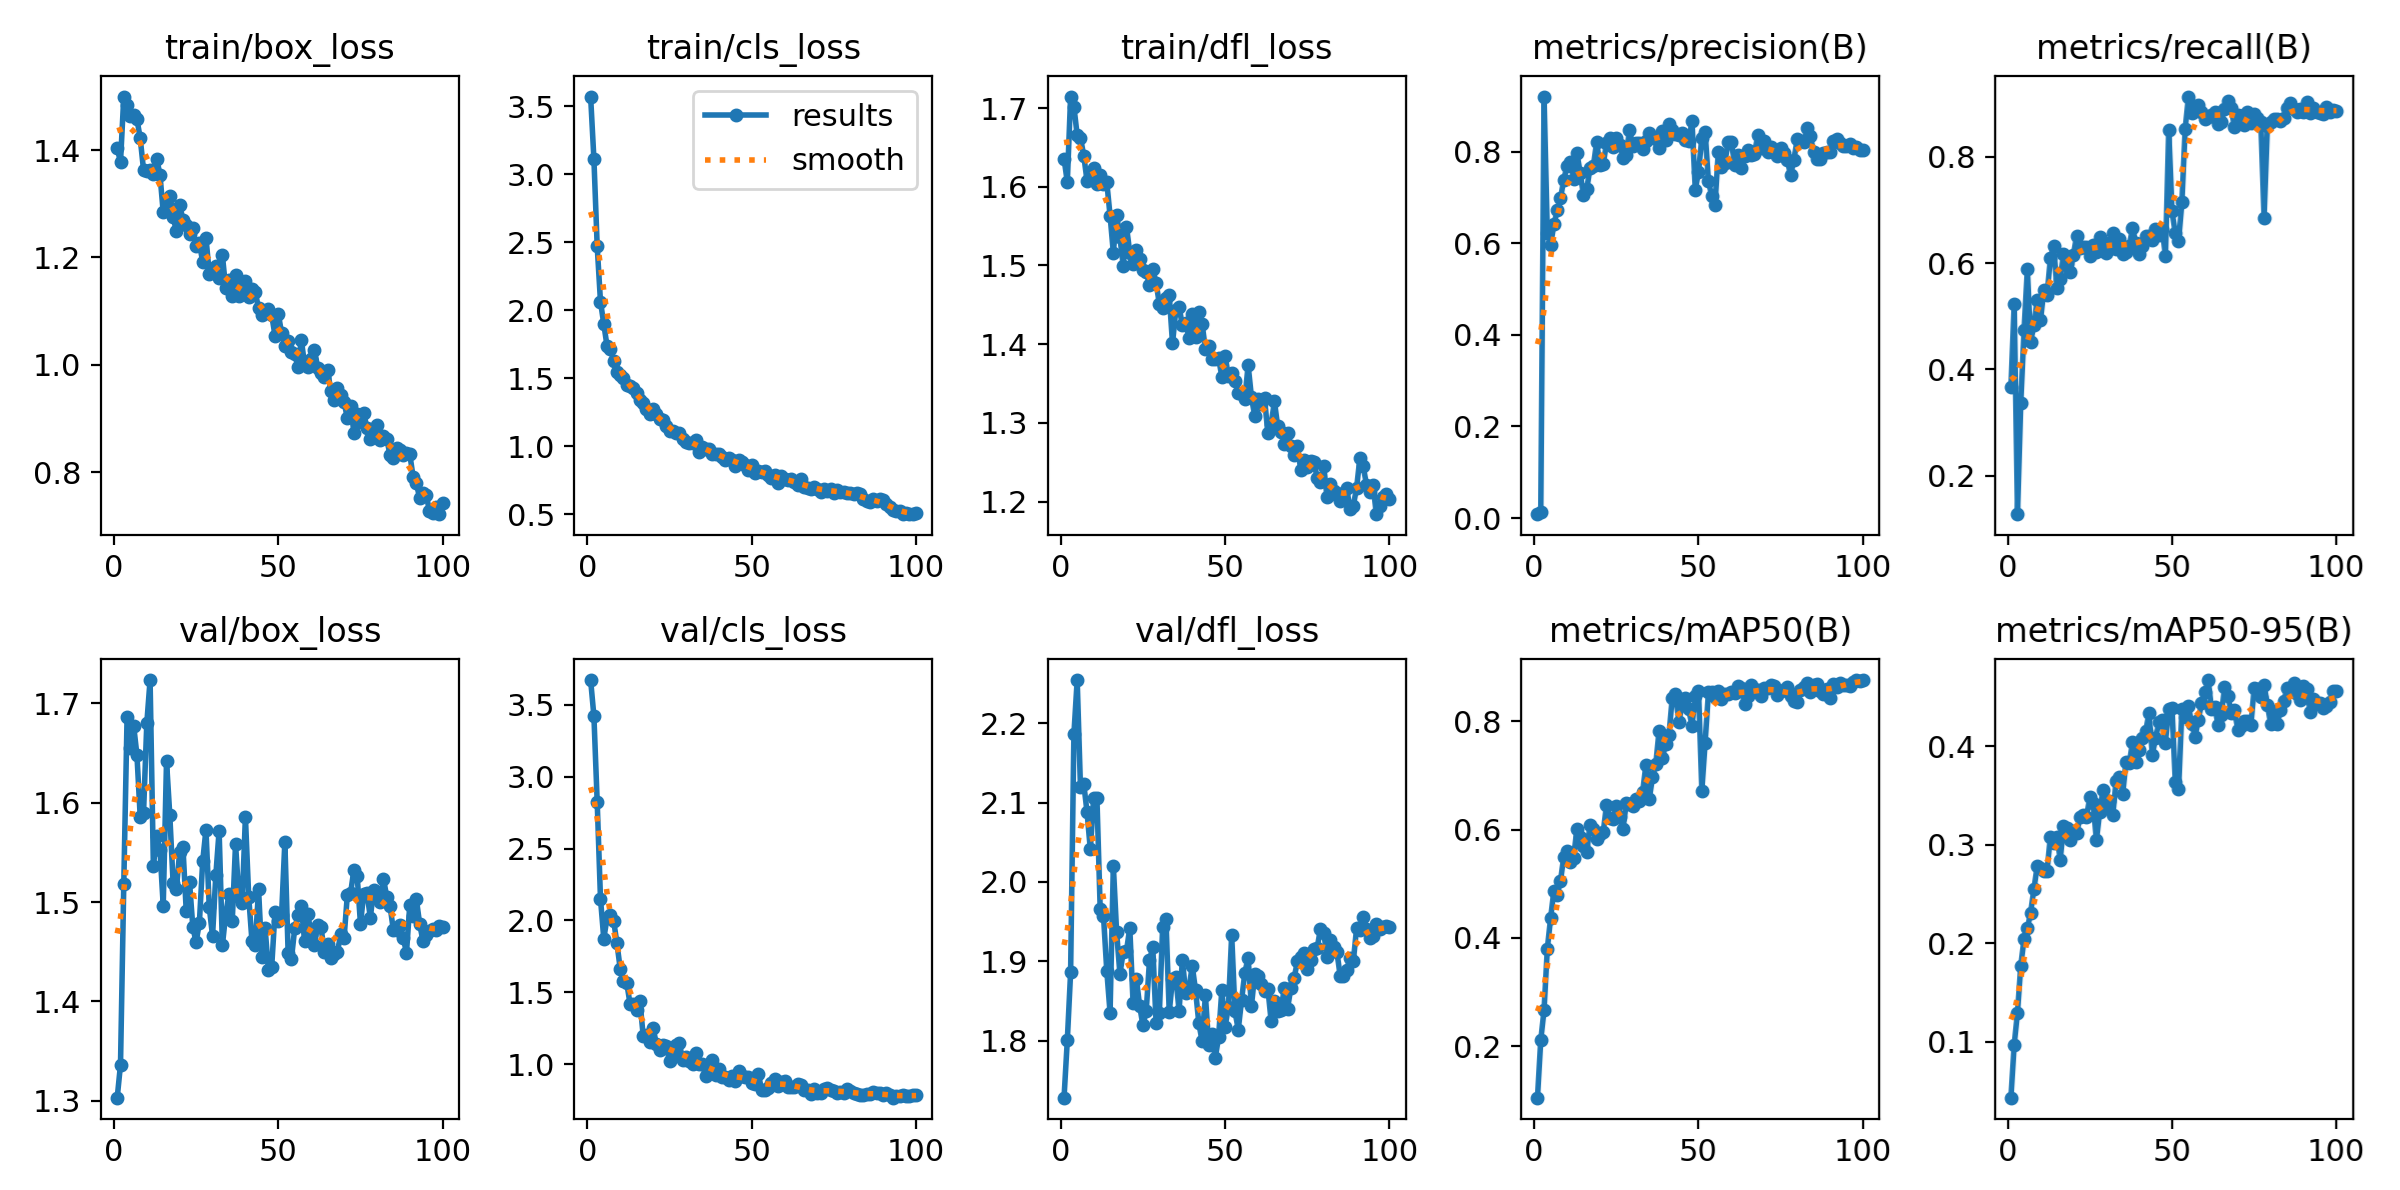
\includegraphics[width=1\linewidth]{Images/yolo11n_accuracy.png}
%     \caption{Accuracy metrics of the original YOLO11n model}
%     \label{fig:yolo11n_accuracy}
% \end{figure}

% \begin{figure}[ht]
%     \centering
%     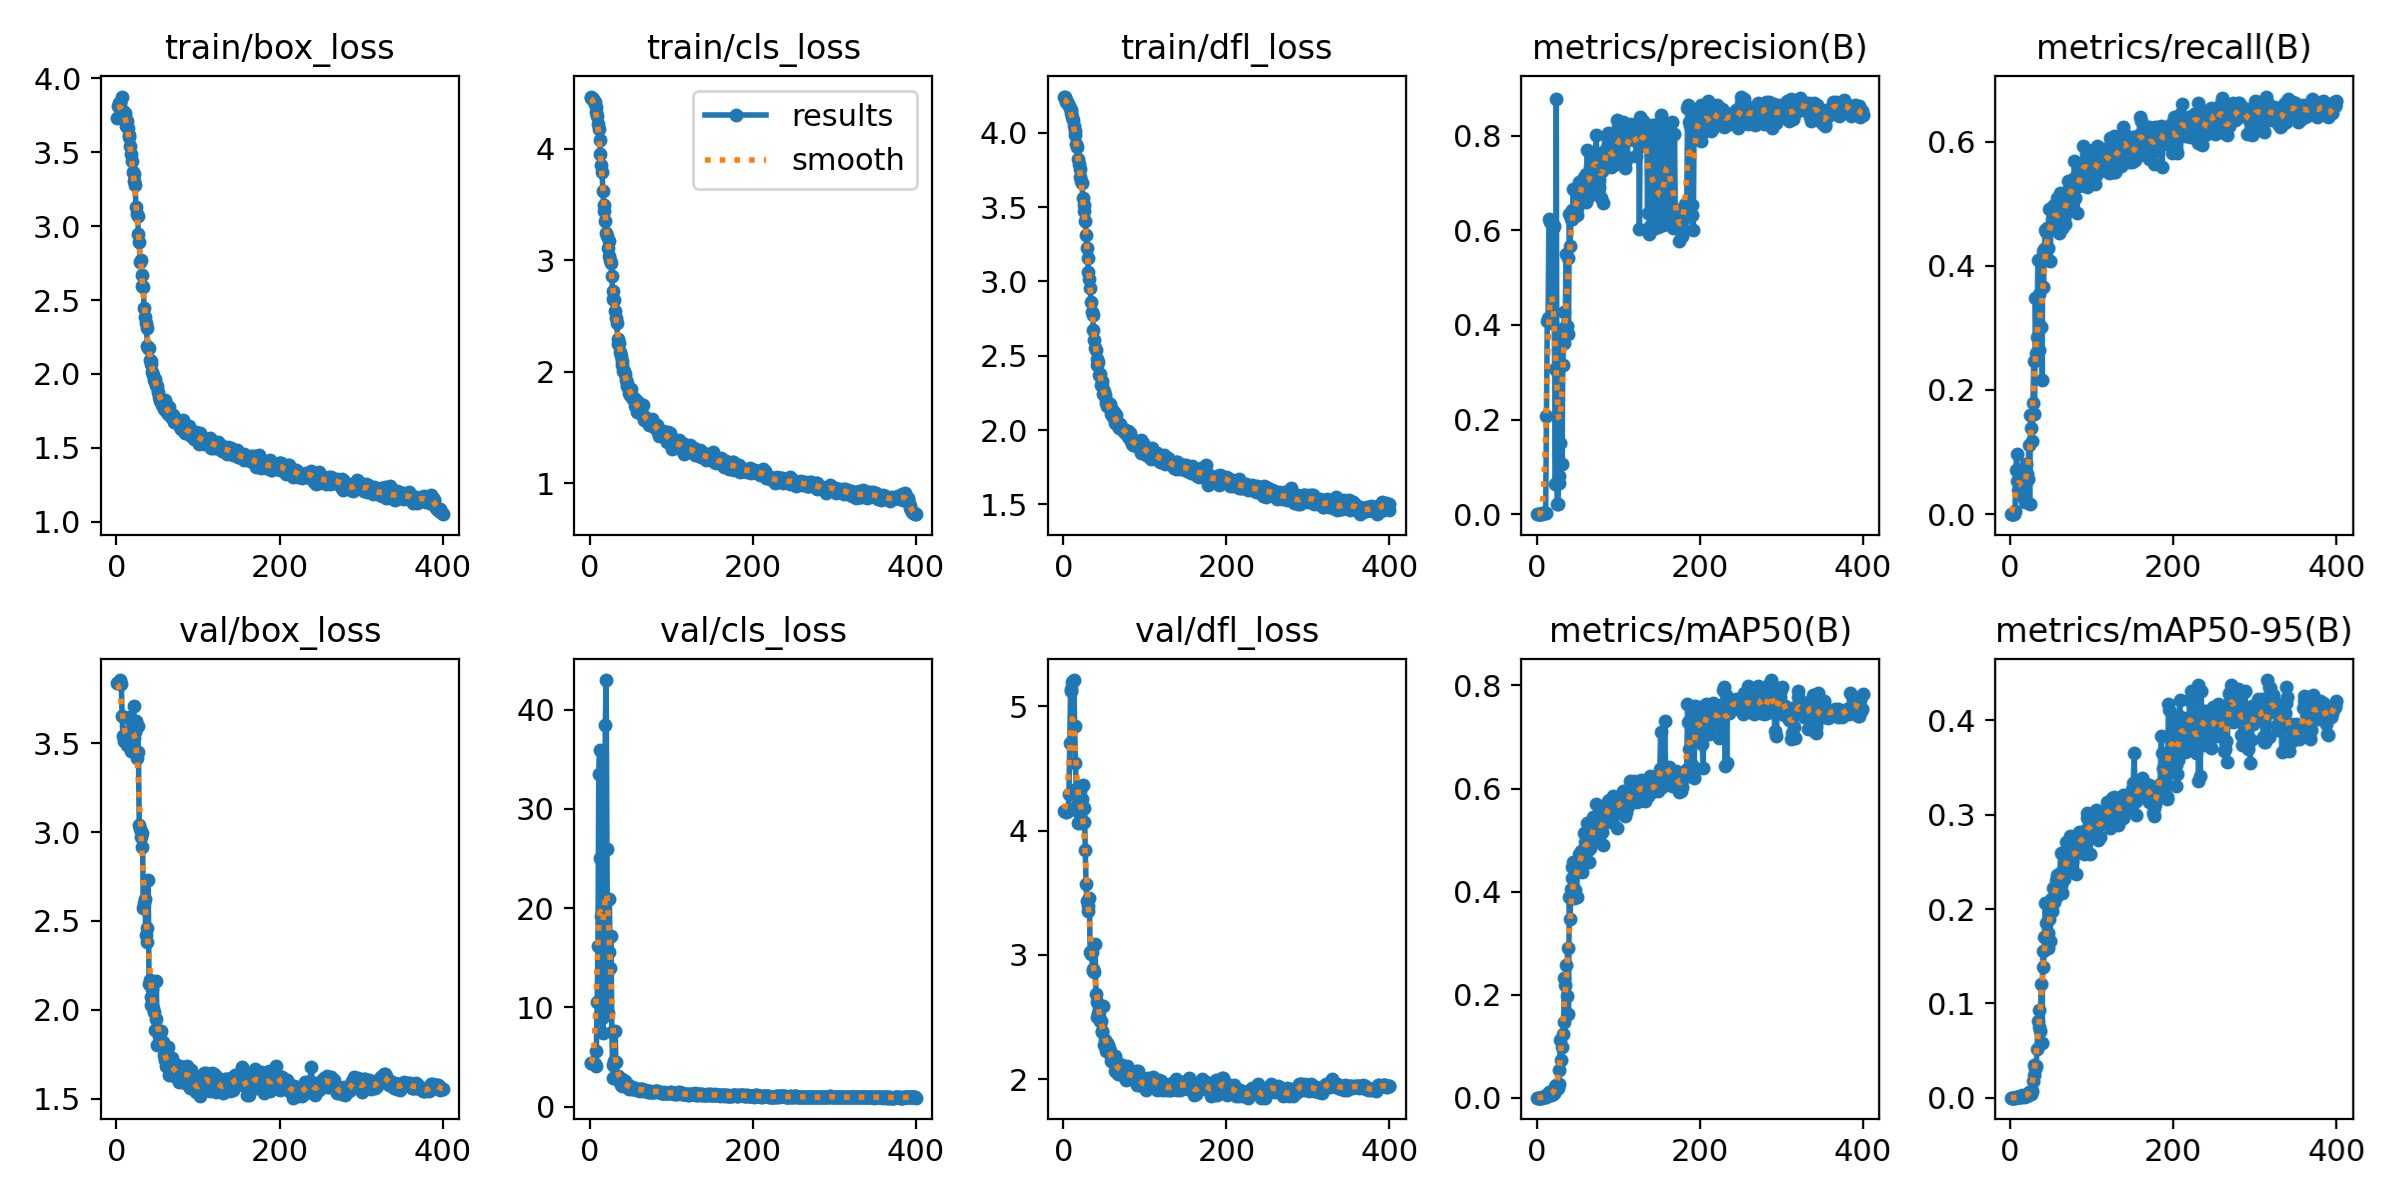
\includegraphics[width=1\linewidth]{Images/yolo11n-mbnv4accuracy.png}
%     \caption{Accuracy metrics of YOLO11n--MobileNetV4 (ConvSmall)}
%     \label{fig:yolo11n-mbnv4_accuracy}
% \end{figure}

% Figures~\ref{fig:yolo11n_accuracy} and \ref{fig:yolo11n-mbnv4_accuracy} show that the original YOLO11n achieves higher detection accuracy, exceeding the MobileNetV4 variant by approximately 10--15\% in both mAP@50 and mAP@50--95. Despite this reduction, the MobileNetV4-based model retains over 85\% of the baseline accuracy, demonstrating stable convergence and sufficient detection performance for traffic light recognition.

% \subsubsection{Inference Speed}

% Inference latency is the primary bottleneck for CPU-based edge deployment. According to official benchmarks, the original YOLO11n (TFLite) requires more than 400\,ms per frame on CPU, resulting in a throughput of only 2--3 FPS \cite{ultralytics_rpi5}.

% In contrast, as summarized in Table~\ref{tab:tradeoff_yolo_models}, the YOLO11n--MobileNetV4 model reduces inference latency to 30--40\,ms, corresponding to a 90--92\% reduction and a 10--13$\times$ speedup. This enables real-time performance of 25--33 FPS on embedded hardware, as illustrated in Fig.~\ref{fig:res_cpp}. The significant latency reduction validates the suitability of the MobileNetV4 backbone for real-time edge inference.

% \begin{table}[ht]
% \centering
% \caption{Performance trade-off between YOLO11n and YOLO11n--MobileNetV4}
% \label{tab:tradeoff_yolo_models}
% \resizebox{\columnwidth}{!}{
% \renewcommand{\arraystretch}{1.3}
% \begin{tabular}{|l|c|c|}
% \hline
% \textbf{Metric} & \textbf{YOLO11n} & \textbf{YOLO11n--MobileNetV4} \\ \hline
% Backbone & CSP-based & MobileNetV4 \\ \hline
% mAP@50 / mAP@50--95 & Higher ($\approx$10--15\%) & Slightly lower \\ \hline
% Inference (CPU) & $>$400 ms & 30--40 ms \\ \hline
% Throughput & 2--3 FPS & 25--33 FPS \\ \hline
% Speedup & 1$\times$ & $\approx$10--13$\times$ \\ \hline
% Edge suitability & Limited & High \\ \hline
% \end{tabular}
% }
% \end{table}


% ----------------------------New section-------------------------
\section{Model Benchmarking}
\label{sec:comparison}

This section evaluates the proposed YOLO11n-MobileNetV4 architecture against the original YOLO11n baseline, focusing on accuracy and inference performance under embedded hardware constraints.

\subsection{Dataset and Hardware Environment}
The proposed model was trained and evaluated on a traffic light dataset comprising approximately 6{,}000 annotated images captured under diverse illumination and environmental conditions, with three target classes: red, yellow, and green. All images were resized to $320 \times 320$ pixels and normalized to the range $[0,1]$ prior to training. Mosaic augmentation was applied to enhance robustness against scale variation and partial occlusion. For deployment experiments, inference was performed on a Raspberry Pi~5 edge device operating in a CPU-only configuration without dedicated GPU or TPU acceleration. The platform is equipped with a Broadcom BCM2712 quad-core Arm Cortex-A76 processor running at 2.4\,GHz, 8\,GB of RAM, and utilizes Google LiteRT as the inference runtime.

\subsection{Compared Models}
Two configurations were evaluated to analyze the speed--accuracy trade-off for embedded traffic light detection:
\begin{itemize}
    \item YOLO11n (original backbone)
    \item YOLO11n--MobileNetV4 (ConvSmall)
\end{itemize}
\subsubsection{Detection Accuracy} 

% \begin{figure}[ht]
%     \centering
%     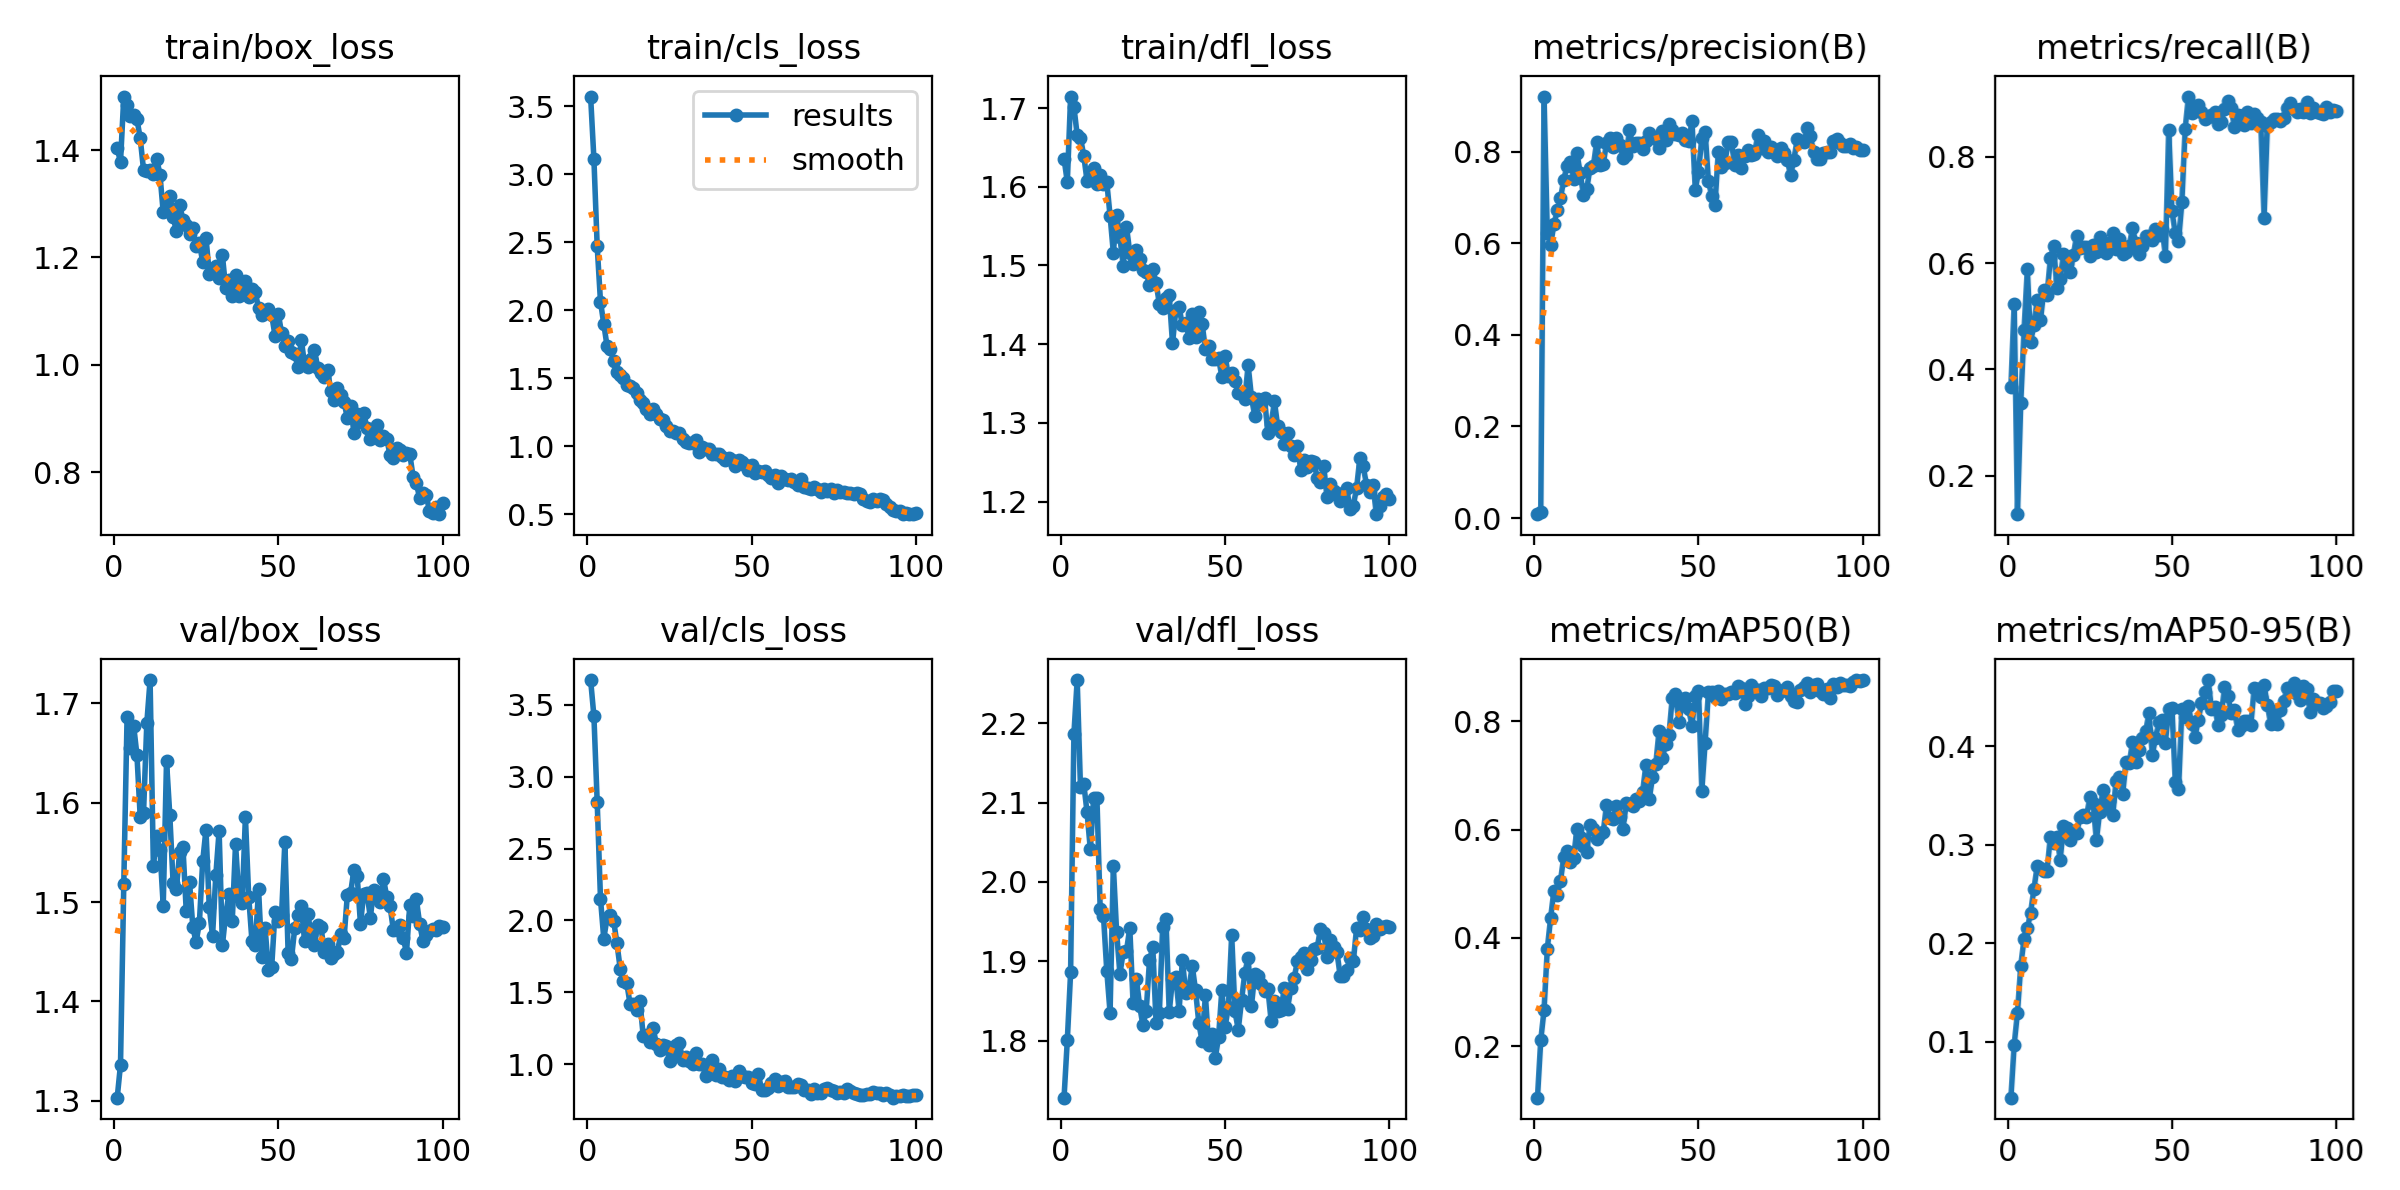
\includegraphics[width=1\linewidth]{Images/yolo11n_accuracy.png}
%     \caption{Accuracy metrics of the original YOLO11n model}
%     \label{fig:yolo11n_accuracy}
% \end{figure}

% \begin{figure}[ht]
%     \centering
%     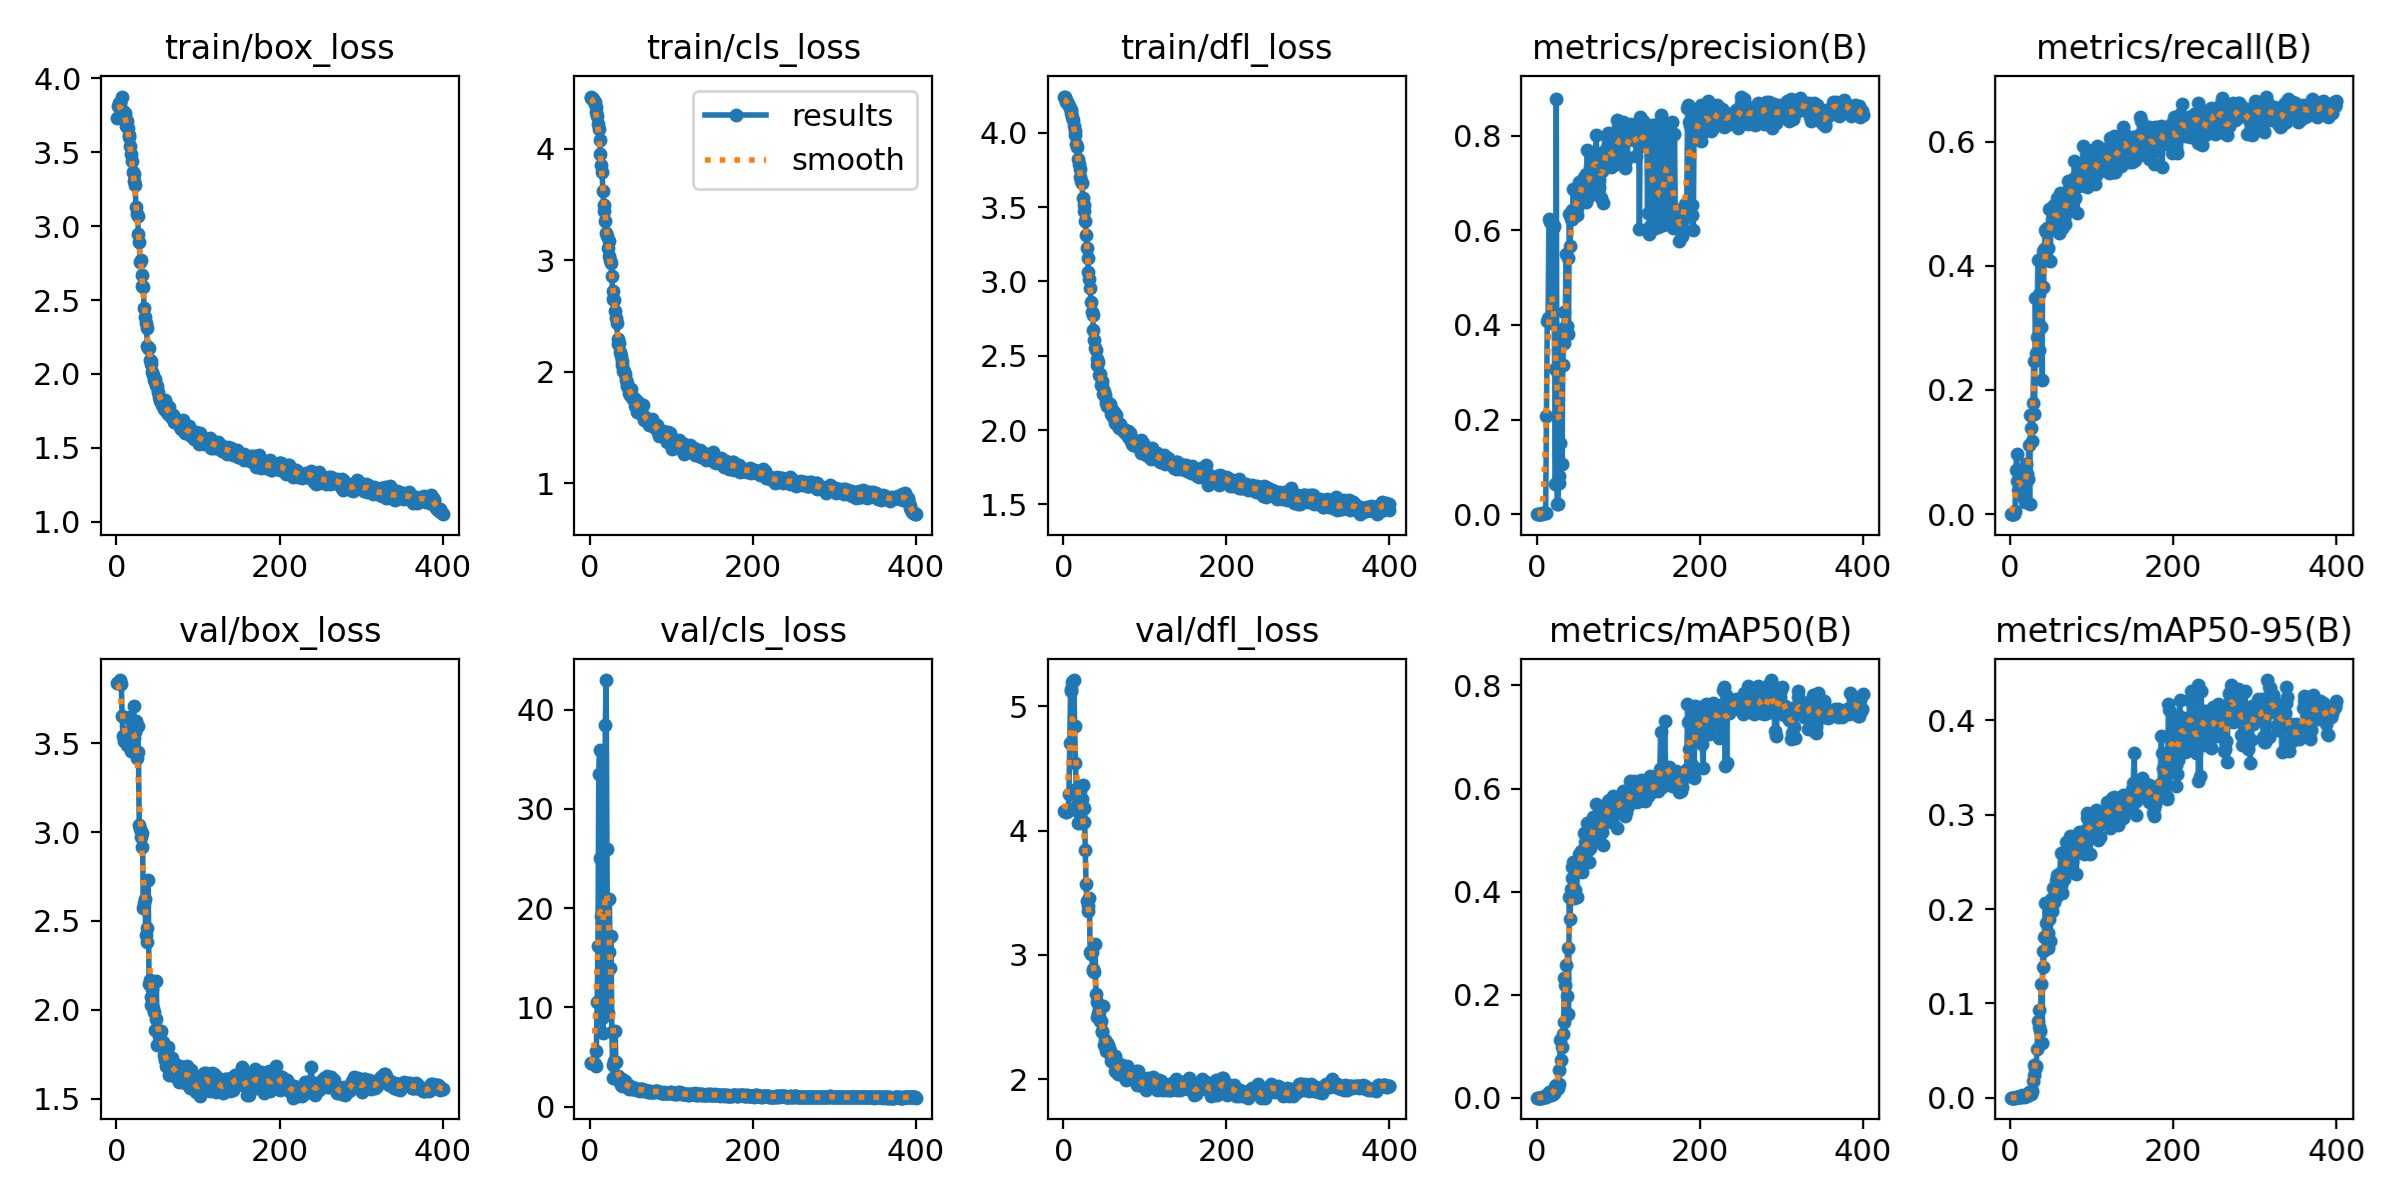
\includegraphics[width=1\linewidth]{Images/yolo11n-mbnv4accuracy.png}
%     \caption{Accuracy metrics of YOLO11n--MobileNetV4 (ConvSmall)}
%     \label{fig:yolo11n-mbnv4_accuracy}
% \end{figure}

\begin{figure}[ht]
    \centering
    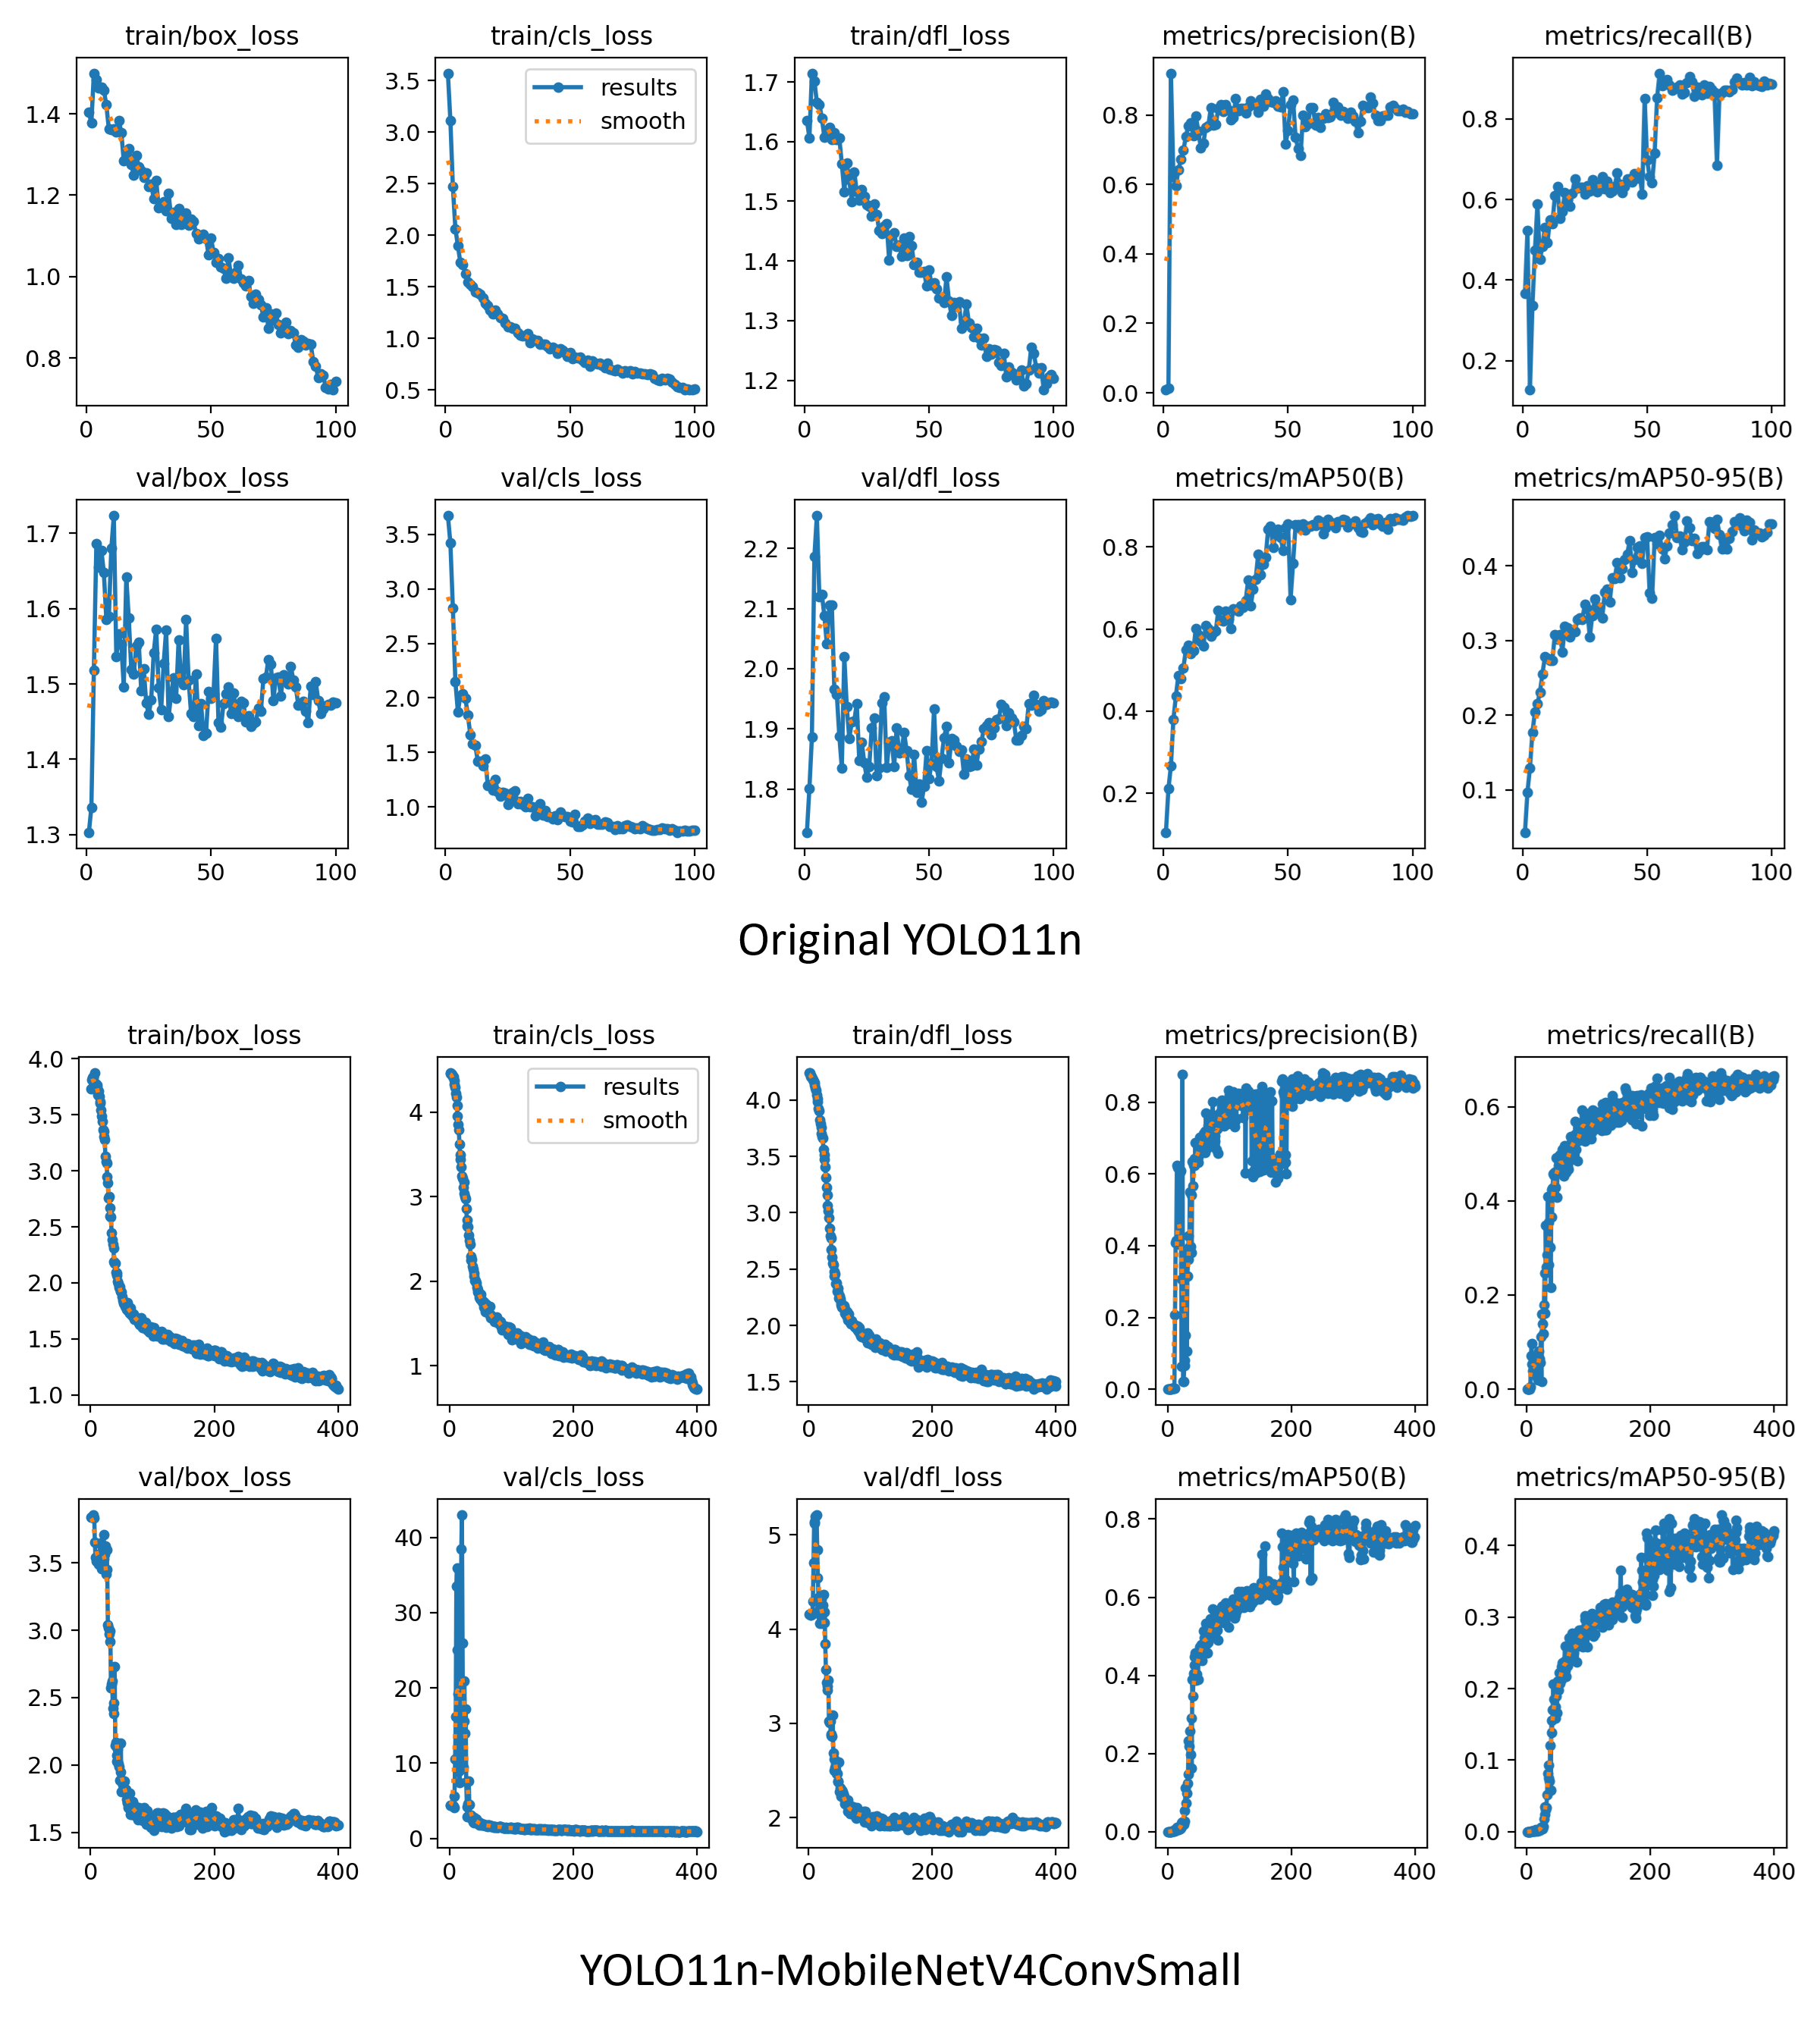
\includegraphics[width=0.9\linewidth]{Images/CompareModel.png}
    \caption{Accuracy metrics of 2 models}
    \label{fig:compare-model}
\end{figure}

% Figures~\ref{fig:yolo11n_accuracy} and \ref{fig:yolo11n-mbnv4_accuracy} show that the original YOLO11n achieves higher detection accuracy, exceeding the MobileNetV4 variant by approximately 10--15\% in both mAP@50 and mAP@50--95. Despite this reduction, the MobileNetV4-based model retains over 85\% of the baseline accuracy, demonstrating stable convergence and sufficient detection performance for traffic light recognition.

Figures \ref{fig:compare-model} shows that the original YOLO11n achieves higher detection accuracy, exceeding the MobileNetV4 variant by approximately 10--15\% in both mAP@50 and mAP@50--95. Despite this reduction, the MobileNetV4-based model retains over 85\% of the baseline accuracy, demonstrating stable convergence and sufficient detection performance for traffic light recognition.


\subsubsection{Inference Speed}

Inference latency is the primary bottleneck for CPU-based edge deployment. According to official benchmarks, the original YOLO11n (TFLite) requires more than 400\,ms per frame on CPU, resulting in a throughput of only 2--3 FPS \cite{ultralytics_rpi5}.

In contrast, as summarized in Table~\ref{tab:tradeoff_yolo_models}, the YOLO11n--MobileNetV4 model reduces inference latency to 30--40\,ms, corresponding to a 90--92\% reduction and a 10--13$\times$ speedup. This enables real-time performance of 25--33 FPS on embedded hardware, as illustrated in Fig.~\ref{fig:res_cpp}. The significant latency reduction validates the suitability of the MobileNetV4 backbone for real-time edge inference.

\begin{table}[ht]
\centering
\caption{Performance trade-off between YOLO11n and YOLO11n--MobileNetV4}
\label{tab:tradeoff_yolo_models}
\resizebox{\columnwidth}{!}{
\renewcommand{\arraystretch}{1.3}
\begin{tabular}{|l|c|c|}
\hline
\textbf{Metric} & \textbf{YOLO11n} & \textbf{YOLO11n--MobileNetV4} \\ \hline
Backbone & CSP-based & MobileNetV4 \\ \hline
mAP@50 / mAP@50--95 & Higher ($\approx$10--15\%) & Slightly lower \\ \hline
Inference (CPU) & $>$400 ms & 30--40 ms \\ \hline
Throughput & 2--3 FPS & 25--33 FPS \\ \hline
Speedup & 1$\times$ & $\approx$10--13$\times$ \\ \hline
Edge suitability & Limited & High \\ \hline
\end{tabular}
}
\end{table}

The experimental results demonstrate the feasibility and efficiency of the proposed approach for real-time traffic light detection on edge devices. Based on these findings, the final section summarizes the key contributions and discusses the implications for future AUTOSAR-based edge perception systems.
